\section{Application: Alpha-to-RGB Generation}
\label{magick_sec:application_alpha_to_rgb}

This dataset has many potential applications It could be used to train a direct RGBA generation method or for training improved matting methods.
To illustrate the usefulness of the dataset, we investigated the application of alpha-to-RGB generation. Given an alpha matte and a prompt as input, we train a model to generate an accompanying RGB image.

\paragraph{Method}
We trained ControlNet~\cite{zhang2023adding} with Stable Diffusion 1.5 (SD1.5) on our dataset. As the output is RGB, we must decide on a background for our target images. We chose to composite our objects onto gray backgrounds. The pure foreground color $F$ can easily be derived with:
\begin{equation} \label{magick_eq:fg}
    F = \frac{1}{\alpha} (I - G) + G
\end{equation}
where $G$ is the color of the gray background. Only $G$ needs to be estimated to compute \cref{magick_eq:fg} which is trivial as the $G$ is nearly constant. Because gray is a neutral color, any small errors in estimating $G$ will not shift the hue of $F$.

We used ControlNet's default settings for training. For testing, we also use the default settings except we set our guidance scale to 7.5 and our control strength to 1.2 as we found empirically this generates better results.

\paragraph{Baselines}
We are unaware of any baselines that directly take alpha and produce a corresponding RGB with adherence to detailed edges. SegGen~\cite{ye2023seggen} proposes a mask-to-image model, but it assumes multiple objects and does not produce matted details. While ControlNet v1.1 can take segmentation masks as guidance, it was trained on ADE20K~\cite{zhou2017scene} and so has a limited set of classes it covers and its adherence to the matted details is too poor to provide a meaningful comparison (see \cref{magick_fig:priorwork} top).

Instead, we convert our mask into edges and compare to ControlNet using canny edges and sketch edges as guidance as proposed in~\cite{zhang2023adding}. For fair comparison, we use SD1.5, the same base model we trained on our dataset.

\begin{figure}
    \centering
    \includegraphics[width=1\linewidth]{src/3_MAGICK/survey.png}
    \caption[User study interface for alpha-to-RGB evaluation]{Interface for user study.}
    \label{magick_fig:user_ui}
\end{figure}

\paragraph{Experiment}
We used the 27 alpha masks from the alphamatting.com training set~\cite{rhemann2009perceptually} as the test set for our experiment. This dataset contains interesting, complex alpha mattes that were not seen by any of the algorithms before testing. Prompts were generated for the images using GPT4. Each method generated three RGB images for each of the 27 examples given their alpha mattes and prompts.

\paragraph{Results}
We asked 52 participants to rate our results verses those from SD1.5 Canny edges and sketch edges. As shown in \cref{magick_fig:user_ui}, the users were presented with the prompt and two row of images, with each row showing results from one randomly chosen method. The users were asked to select the better row of images according to their appearance and adherence to the prompt. As shown in Table~\ref{magick_tab:user_results}, our results were preferred 82\% of the time over SD1.5 Canny Edges and 77\% of the time over SD1.5 Sketch edges. \cref{magick_fig:user_results} shows example results from our experiment.  Despite differences from the original image (shown for reference and not used in the study), the model trained with our dataset is able to create aesthetically pleasing objects that follow the given alpha. The captions and results from all three methods are shown in the Appendix.



\cref{magick_fig:S} shows examples of our alpha-to-rgb generation. The mask of the letter ``S'' was given to our model along with eight different captions to create a number stylized glyphs. The shapes of the generated letters conform to the input mask. Despite not being explicitly trained for glyph generation, the model produced a variety of aesthetically pleasing results. Surprisingly, several results show consistent 3d effects such as realistic extrusion or shadowing (e.g. the top left and bottom right examples). Semantic features also emerged, such as the cookie and pizza examples both showing overcooking along the edges of the glyphs but not the interiors as can happen with real food.

\begin{table}[!t]
  \centering
  \begin{tabular}{r|cc}
    \toprule
     & \multicolumn{2}{c}{User preference}  \\
    SD guidance & SD1.5 & Ours \\
    \midrule
    Canny Edges & .16 & \textbf{.82} \\
    Sketch Edges & .23 & \textbf{.77} \\
    \bottomrule
  \end{tabular}
   \caption[User study results for alpha-to-RGB generation]{Results of user study on alpha-to-rgb generation.}\label{magick_tab:user_results}
\end{table}

\begin{figure}
    \centering
    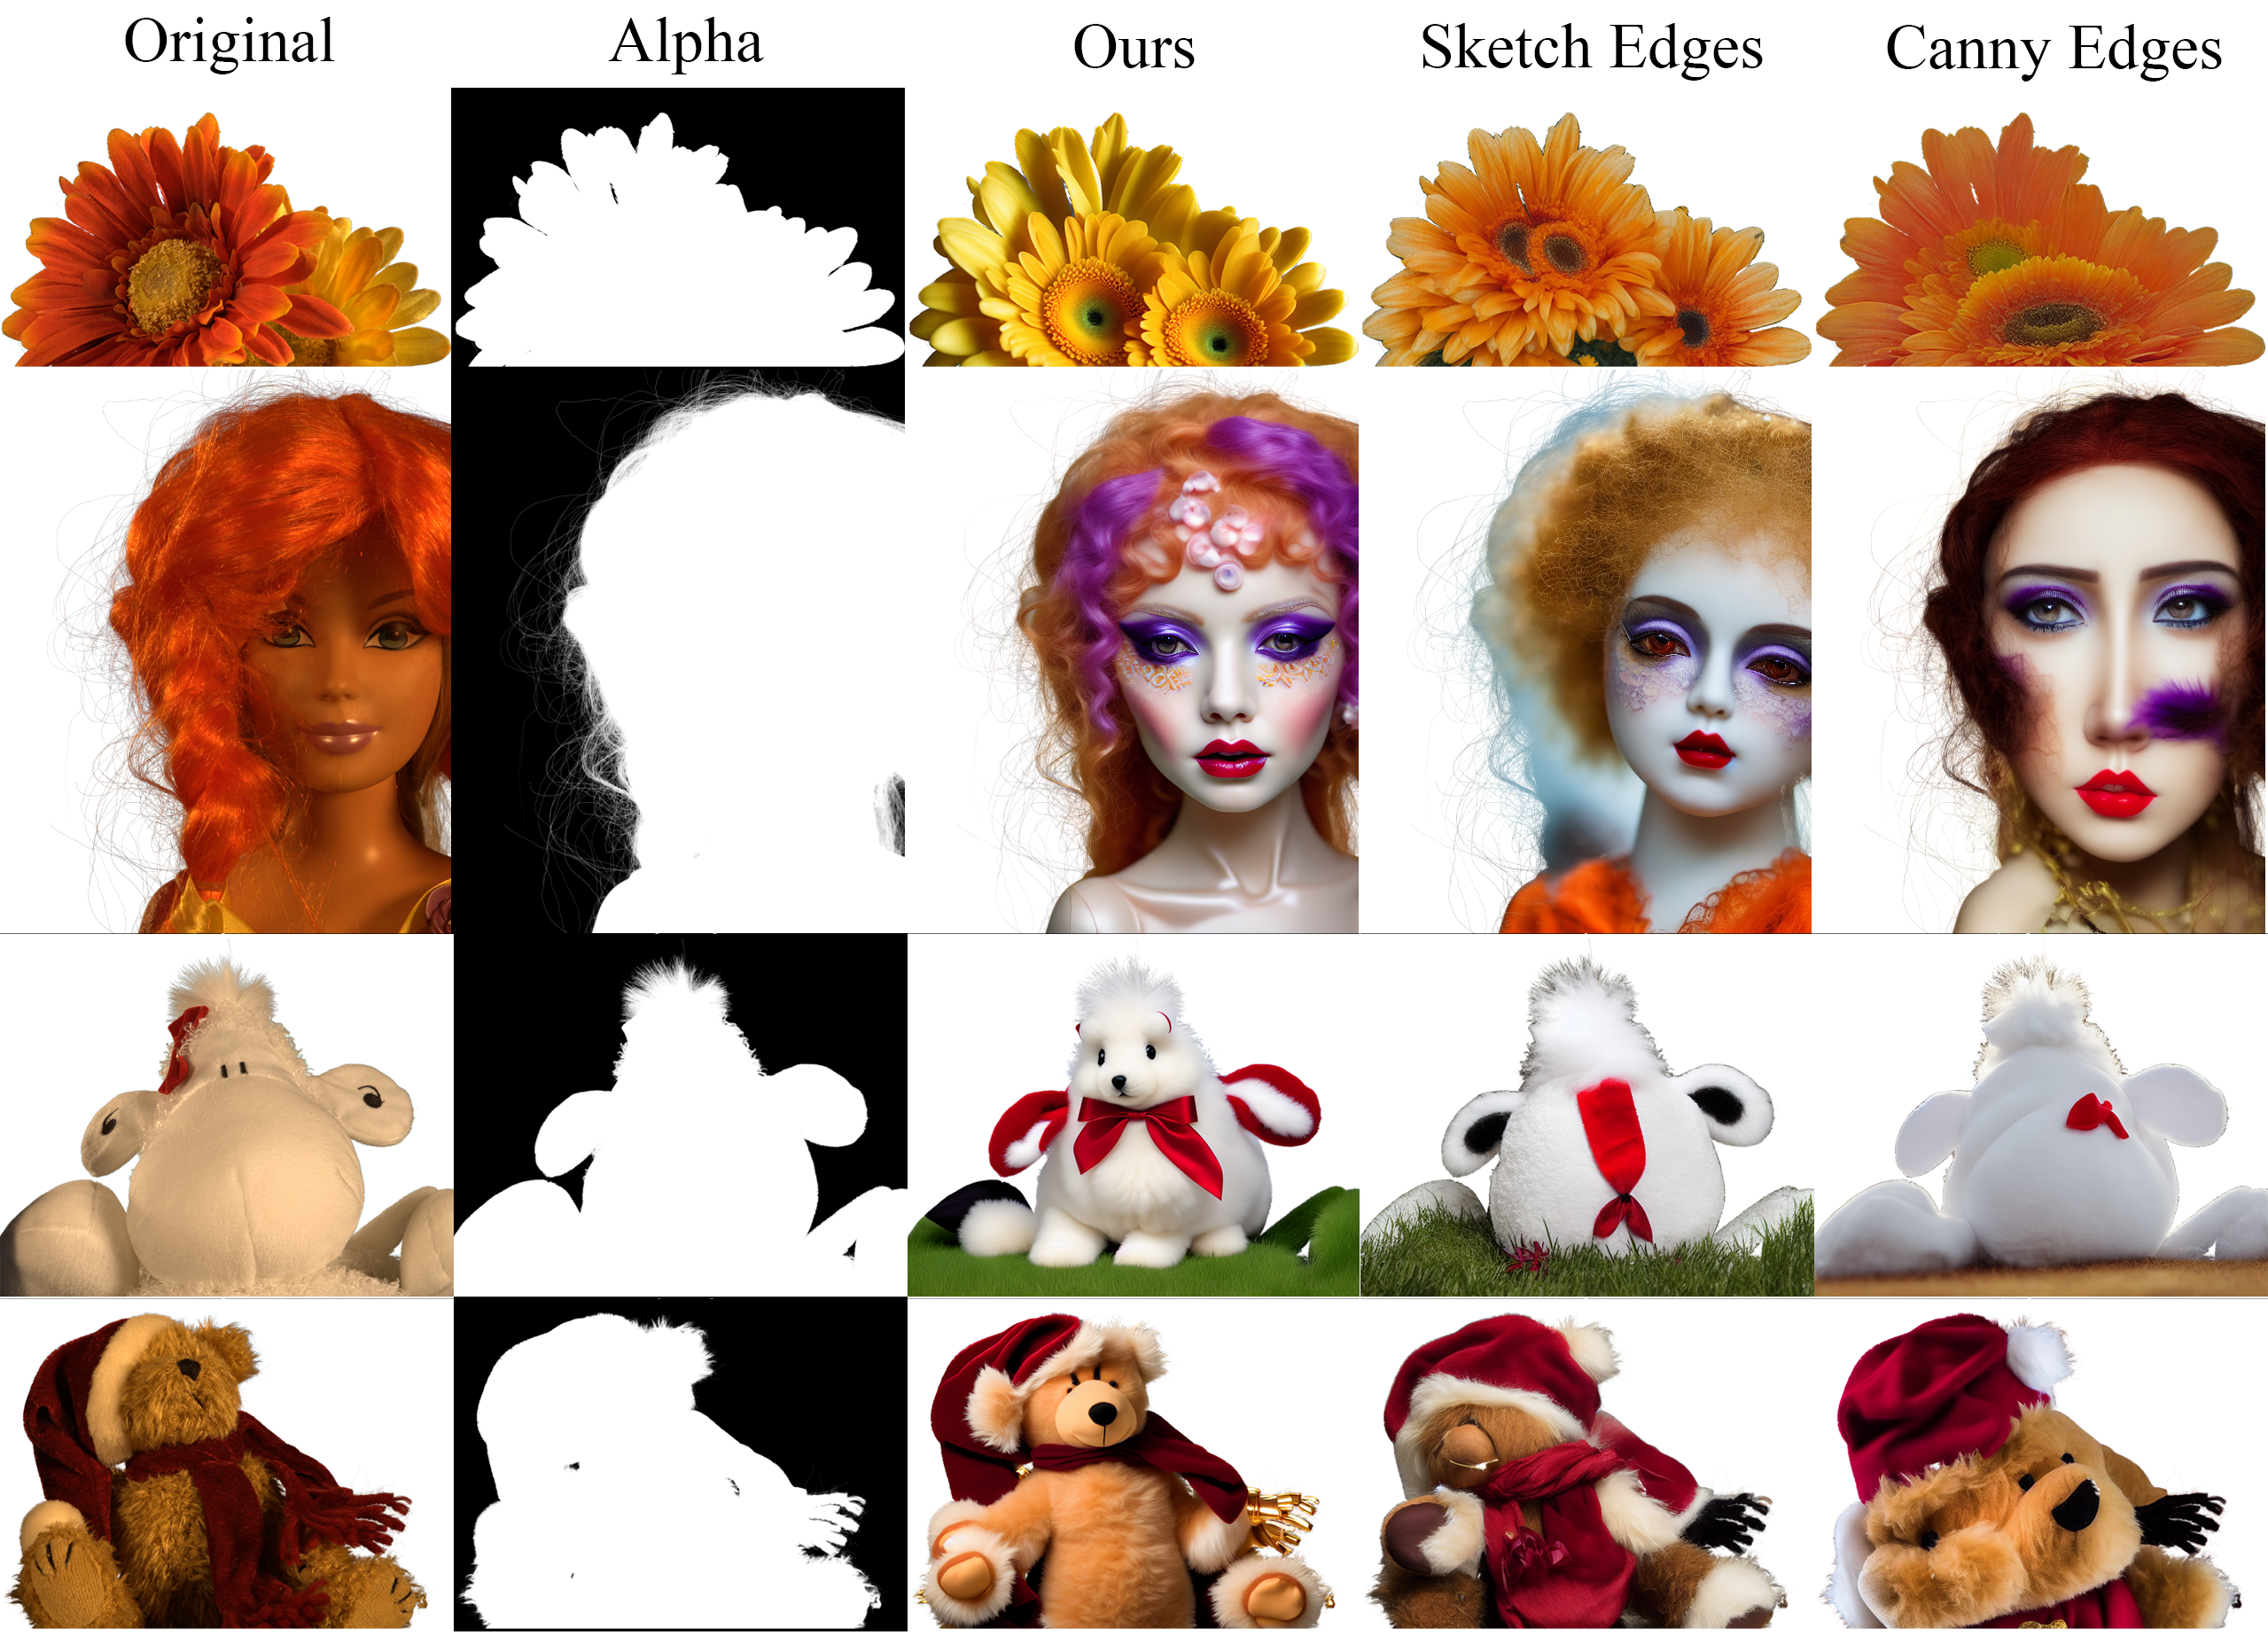
\includegraphics[width=1\linewidth]{src/3_MAGICK/figs/alpha2rgbResults.png}
    \caption[Alpha-to-RGB generation results from user study]{Generation results from our user study. The original images were the original images from~\cite{rhemann2009perceptually}, shown as reference and not used in the study. Given the alpha values and captions (not shown), images were generated using SD1.5 trained with our dataset, SD1.5 Sketch Edges, and SD1.5 Canny edges. }
    \label{magick_fig:user_results}
\end{figure}



\begin{figure}
    \centering
    \includegraphics[width=1\linewidth]{src/3_MAGICK/figs/S3.png}
    \caption[Stylized glyph generation using alpha-to-RGB]{Example of alpha-to-rgb generation. The letter ``S'' is generated using different prompts to generate stylized text.}
    \label{magick_fig:S}
\end{figure}
